% Created 2021-09-10 Fri 23:31
% Intended LaTeX compiler: pdflatex
\documentclass[bigger]{beamer}
\usepackage[utf8]{inputenc}
\usepackage[T1]{fontenc}
\usepackage{graphicx}
\usepackage{grffile}
\usepackage{longtable}
\usepackage{wrapfig}
\usepackage{rotating}
\usepackage[normalem]{ulem}
\usepackage{amsmath}
\usepackage{textcomp}
\usepackage{amssymb}
\usepackage{capt-of}
\usepackage{hyperref}
\usepackage{pifont}
\usepackage{verbatim}
\makeatletter
\def\verbatim@font{\scriptsize\ttfamily}
\makeatother
\logo{
\includegraphics[height=0.5cm]{./img/usp-logo-1}}
\usetheme[height=20pt]{Madrid}
\usecolortheme{seahorse}
\author{Pedro G. Branquinho}
\date{  Universidade de São Paulo - DEMAR}
\title{O \LaTeX{} e alguns modelos}
\setbeamertemplate{itemize item}{\ding{166}}
\setbeamercolor{item projected}{bg=magenta!90!black,fg=white}
\setbeamertemplate{enumerate item}[circle]
\setbeamercolor{block title}{bg=red!30!white,fg=black}
\hypersetup{
 pdfauthor={Pedro G. Branquinho},
 pdftitle={O \LaTeX{} e alguns modelos},
 pdfkeywords={},
 pdfsubject={},
 pdfcreator={Emacs 27.2 (Org mode 9.4.4)}, 
 pdflang={Portuguese}}
\begin{document}

\maketitle
\begin{frame}{Outline}
\tableofcontents
\end{frame}


\section{Sumário de tópicos}
\label{sec:orgfc92593}
\subsection{Pioneiros e Fundadores}
\label{sec:orgd3cd4f3}
\begin{frame}[label={sec:org798d10f},fragile]{Origem de \TeX{} - Knuth (1978)}
 \begin{columns}
\begin{column}{0.48\columnwidth}
\begin{block}<1->{Imagem do Knuth}
\href{img/KnuthAtOpenContentAlliance.jpg}{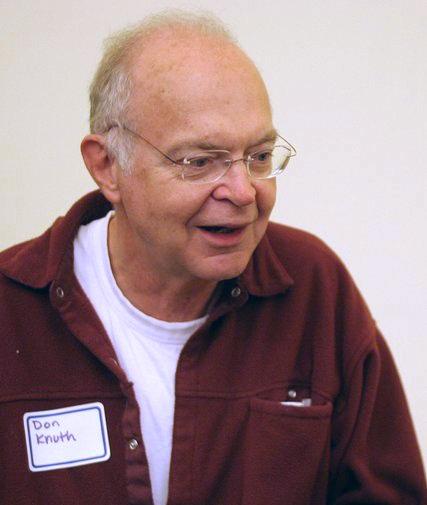
\includegraphics[center,width=1.02\textwidth]{/home/buddhilw/PP/LaTeX/SEMEF-minicurso/Apres1/img/KnuthAtOpenContentAlliance.jpg}}
\end{block}
\end{column}
\begin{column}{0.48\columnwidth}
\begin{block}<1->{Código Imagem}
\begin{verbatim}
\begin{figure}[!ht]
  \centering
  \includegraphics[width=\linewidth]
                  {./img/Knuth.png}
\end{figure}
\end{verbatim}
\end{block}
\end{column}
\end{columns}
\end{frame}


\begin{frame}[label={sec:org07dec03},fragile]{Roupagem moderna, \LaTeX{} - Leslie Lamport (1985)}
 \begin{columns}
\begin{column}{0.48\columnwidth}
\begin{block}<1->{Imagem Lamport}
\href{img/Leslie\_Lamport.jpg}{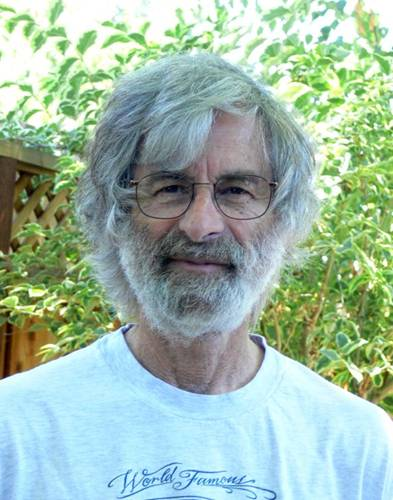
\includegraphics[center,width=1.02\textwidth]{./img/Leslie_Lamport.jpg}}
\end{block}
\end{column}
\begin{column}{0.48\columnwidth}
\begin{block}<1->{Código da Imagem}
\begin{verbatim}
\begin{figure}[!ht]
  \centering
  \includegraphics[width=\linewidth]
                  {./img/Lamport.png}
\end{figure}
\end{verbatim}
\end{block}
\end{column}
\end{columns}
\end{frame}

\subsection{Aplicações que utilizam de \LaTeX{}}
\label{sec:orgaa1ea78}
\begin{frame}[label={sec:org1a9b151}]{MathJax - \LaTeX{} na Web}
\href{img/mathjax.png}{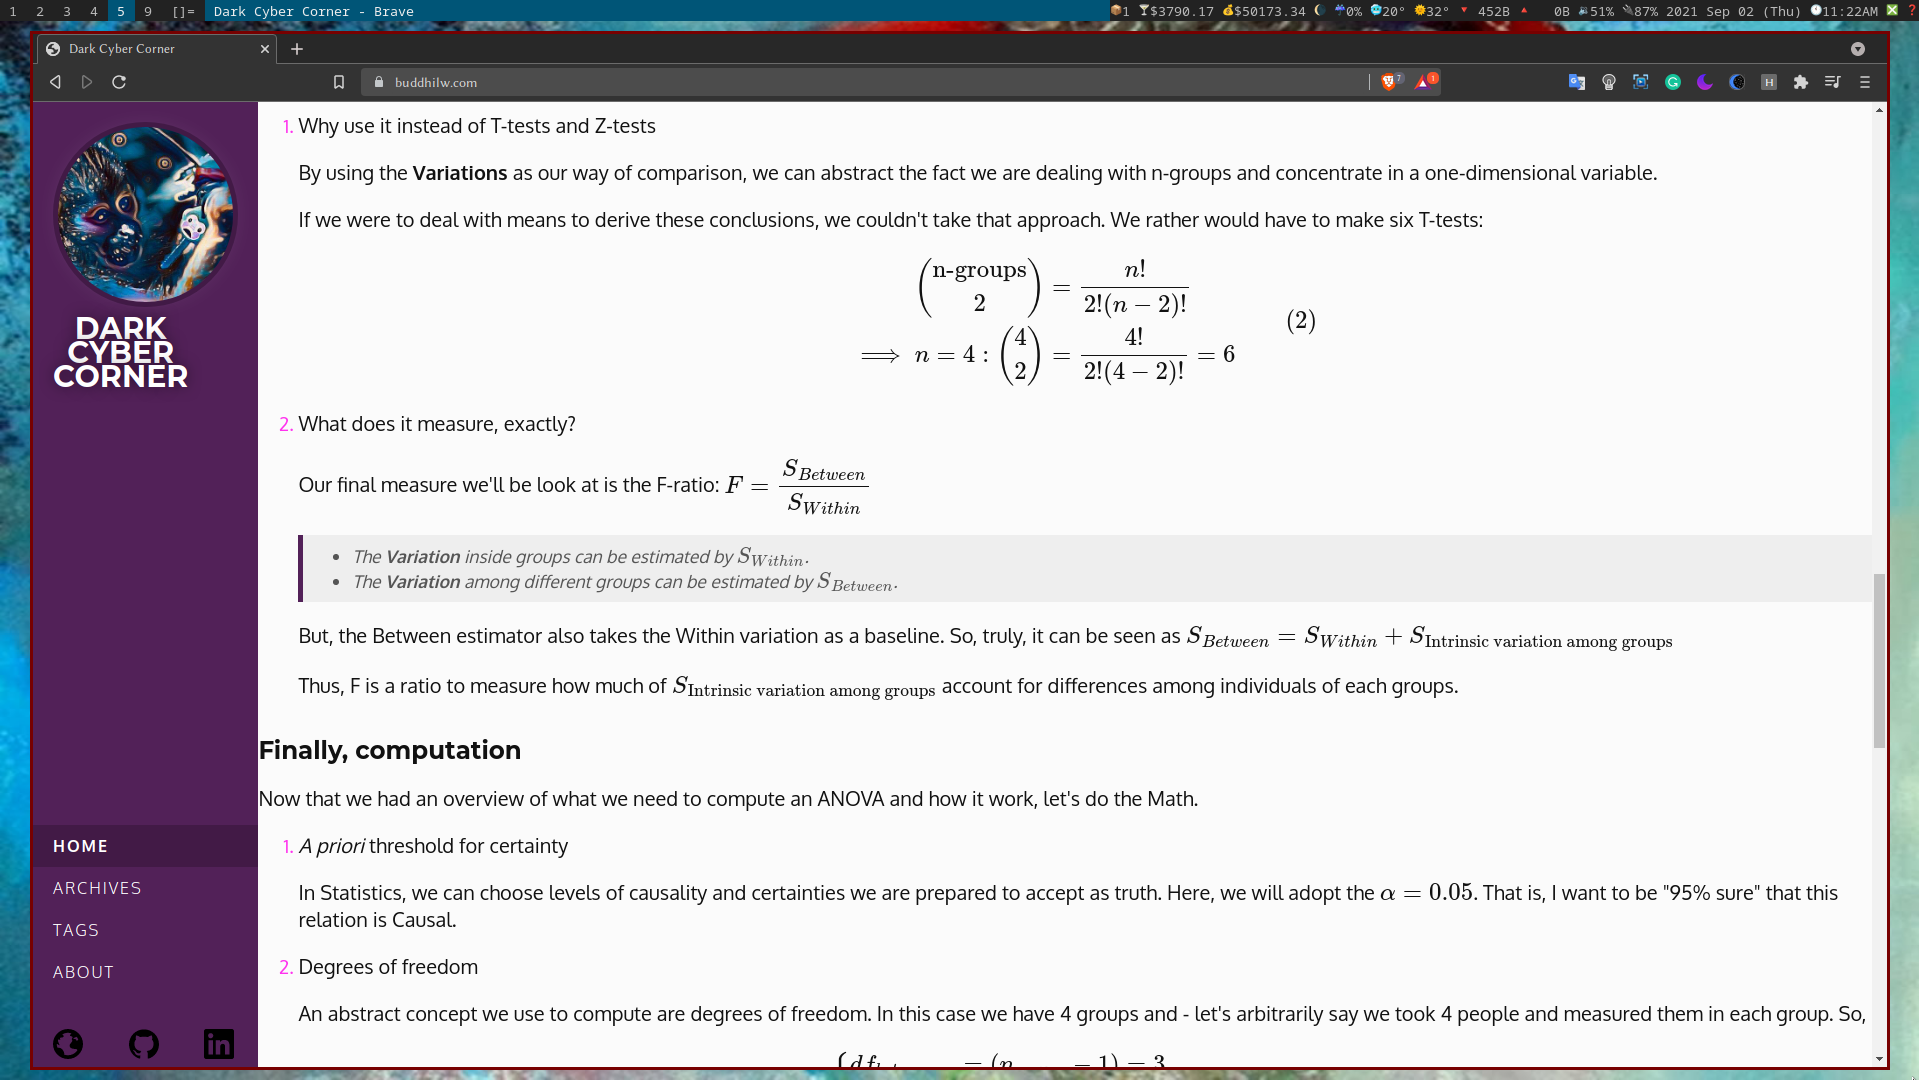
\includegraphics[center,width=1.02\textwidth]{/home/buddhilw/PP/LaTeX/SEMEF-minicurso/Apres1/img/mathjax.png}}
\end{frame}


\begin{frame}[label={sec:org42f7375},fragile]{Org-mode e AUCTeX (O código que usamos)}
 \begin{block}<1->{Código da Equação de Navier-Stokes}
\begin{verbatim}
\begin{equation}
        \begin{aligned}
        \dfrac{\partial{\vec{V}}}{\partial{t}}
        + \vec{V}.\nabla{\vec{V}}
        = - \dfrac{\nabla{p}}{\rho}
        + \nu{}\nabla^2{\vec{V}}
        \end{aligned}
\end{equation}
\end{verbatim}
\end{block}

\begin{block}<1->{Renderização Equação de Navier-Stokes}
\begin{equation}
        \begin{aligned}
        \dfrac{\partial{\vec{V}}}{\partial{t}} + \vec{V}.\nabla{\vec{V}} = - \dfrac{\nabla{p}}{\rho} + \nu{}\nabla^2{\vec{V}}
        \end{aligned}
\end{equation}
\end{block}
\end{frame}

\begin{frame}[label={sec:org90805ea}]{Dentro do Org-mode, no Emacs}
\begin{itemize}[<+->]
\item Preview em tempo real.
\item Aparência customizável.
\item Ecossistema para programação.
\end{itemize}

\href{img/orgmode-auctex.png}{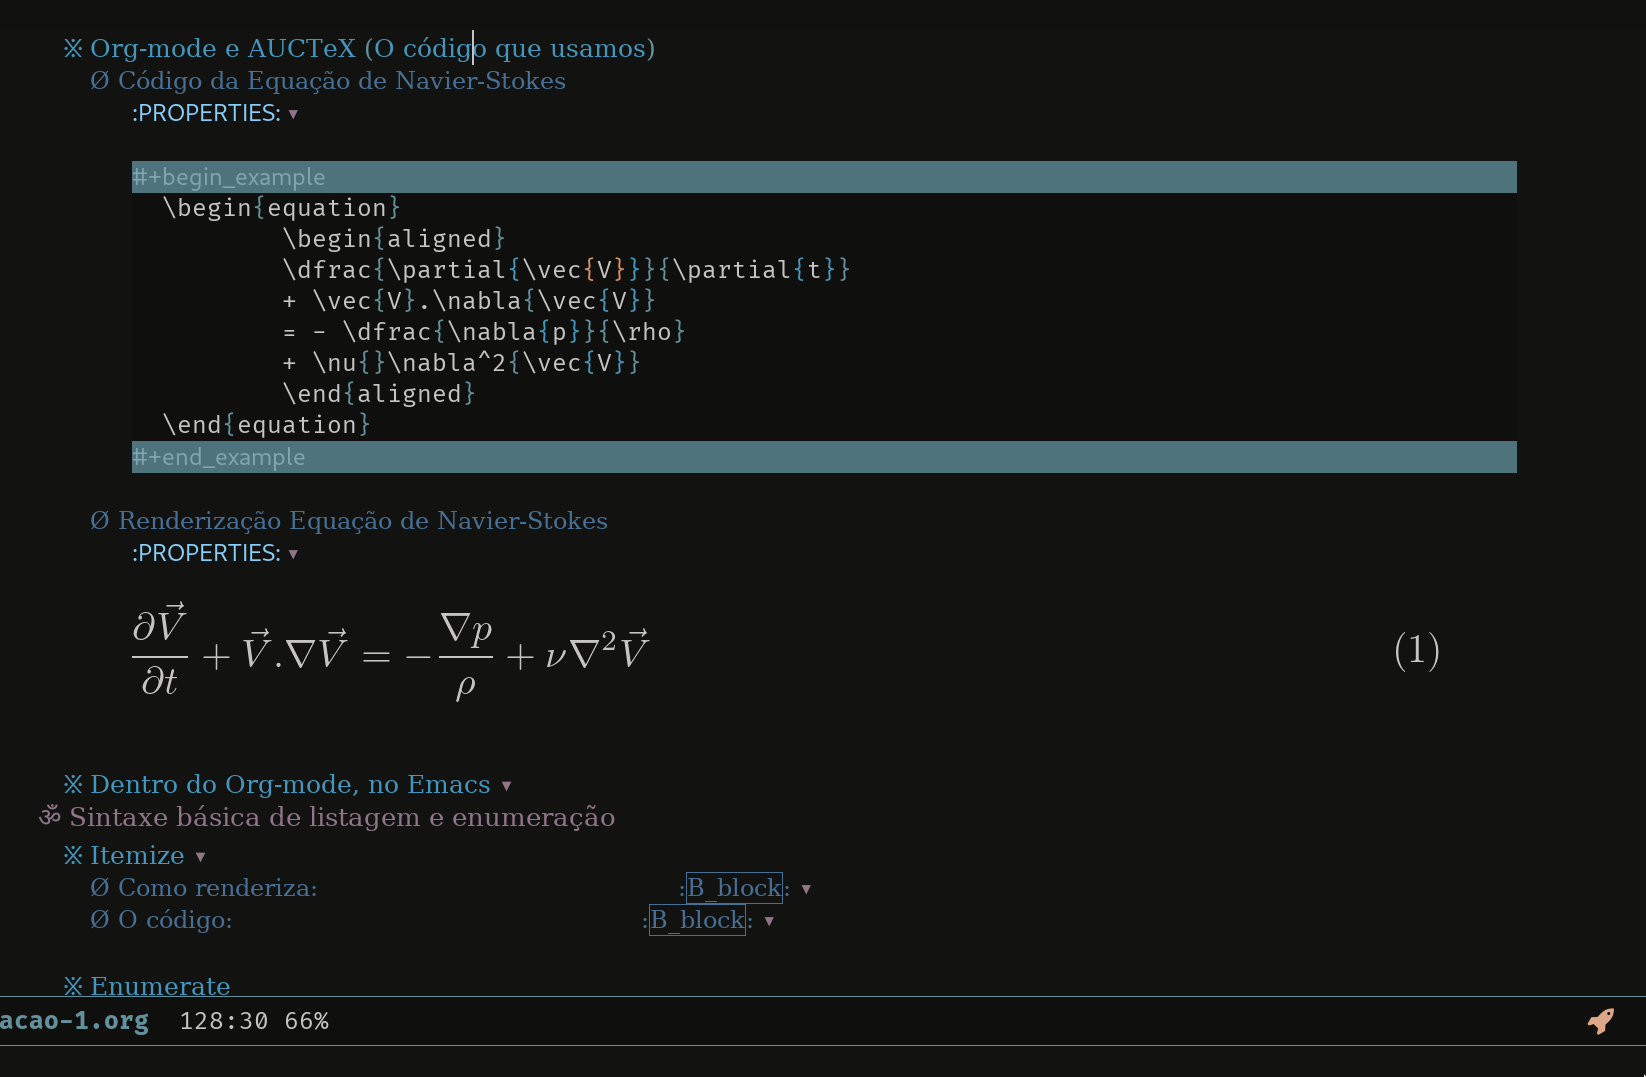
\includegraphics[center,width=0.8\textwidth]{./img/orgmode-auctex2.png}}
\end{frame}

\subsection{Sintaxe básica de listagem e enumeração}
\label{sec:org1ad3d4b}
\begin{frame}[label={sec:org98faf70},fragile]{Itemize}
 \begin{columns}
\begin{column}{0.48\columnwidth}
\begin{block}<1->{Como renderiza:}
\begin{itemize}
\item Primeiro item
\item Segundo item
\end{itemize}
\end{block}
\end{column}

\begin{column}{0.48\columnwidth}
\begin{block}<2->{O código:}
\begin{verbatim}
\begin{enumerate}
\item Primeiro item
\item Segundo item
\end{enumerate}
\end{verbatim}
\end{block}
\end{column}
\end{columns}
\end{frame}


\begin{frame}[label={sec:org5116f10},fragile]{Enumerate}
 \begin{columns}
\begin{column}{0.48\columnwidth}
\begin{block}<1->{Como renderiza:}
\begin{enumerate}
\item Primeiro item
\item Segundo item
\end{enumerate}
\end{block}
\end{column}
\begin{column}{0.48\columnwidth}
\begin{block}<2->{O código:}
\begin{verbatim}
\begin{enumerate}
\item Primeiro item
\item Segundo item
\end{enumerate}
\end{verbatim}
\end{block}
\end{column}
\end{columns}
\end{frame}

\subsection{Tabelas}
\label{sec:org2f95c72}
\begin{frame}[label={sec:orgeb75ea4},fragile]{Tabela Simples}
 \begin{block}<1->{Exemplo}
\begin{center}
\begin{tabular}{lll}
\hline
Coluna 1 & Coluna 2 & Coluna 3\\
\hline
\(a_{11}\) & \(a_{12}\) & \(a_{13}\)\\
\(a_{21}\) & \(a_{22}\) & \(a_{23}\)\\
Texto 1 & Texto 2 & Texto 3\\
dsda & dsad & dasdas\\
\hline
\end{tabular}
\end{center}
\end{block}

\begin{block}<2->{Código}
\begin{verbatim}
\begin{center}
  \begin{tabular}{lll}
    \hline
    Coluna 1 & Coluna 2 & Coluna 3\\
    \hline
    \(a_{11}\) & \(a_{12}\) & \(a_{13}\)\\
    \(a_{21}\) & \(a_{22}\) & \(a_{23}\)\\
    Texto 1 & Texto 2 & Texto 3\\
    \hline
  \end{tabular}
\end{center}
\end{verbatim}
\end{block}
\end{frame}
\section{Exemplos de documentos completos}
\label{sec:org4767aaf}
\subsection{Preâmbulo}
\label{sec:org4466d6b}
\begin{frame}[label={sec:orgf9839c3},fragile]{Preâmbulo mínimo}
 \begin{itemize}
\item Onde fica as especificações da tipografia do documentos.
\item Ambiente mais genérico.
\item Onde os comportamentos padrões são especificados.
\end{itemize}
\begin{block}<2->{Definindo a classe do documento}
\begin{verbatim}
%!Tex TS-program = xelatex
%!TEX encoding = UTF-8 Unicode

  \documentclass[
  12pt,				% tamanho da fonte
  openright,			% capítulos começam em pág ímpar (insere página vazia caso preciso)
  oneside,			% para impressão em recto e verso. Oposto a oneside
  a4paper,			% tamanho do papel.
  brazil,				% o último idioma é o principal do documento
  english,			% idioma adicional para hifenização
  ]{abntex2}
  \RequireXeTeX %Force XeTeX check
\end{verbatim}
\end{block}
\end{frame}

\begin{frame}[label={sec:org7fb801d},fragile]{Os pacotes a serem utilizados}
 \begin{block}<1->{Alguns que definem fonte, indentação, etc.}
\begin{verbatim}
% --- (tudo que vem depois de '%' é um comentário em latex)
% PACKAGES
% ---

% ---
% Fundamental Packages
% ---
\usepackage{lmodern}			% Usa a fonte Latin Modern
\usepackage[T1]{fontenc}		% Selecao de codigos de fonte.
\usepackage[utf8]{inputenc}		% Codificacao do documento (conversão automática dos acentos)
\usepackage{indentfirst}		% Indenta o primeiro parágrafo de cada seção.
\usepackage{color}				% Controle das cores
\usepackage{graphicx}			% Inclusão de gráficos
\usepackage{microtype} 			% para melhorias de
% justificação
\usepackage{lipsum}
\usepackage[alf]{abntex2cite}	% Citações padrão ABNT
\usepackage{amsmath}            % Ambientes matemáticos
\end{verbatim}
\end{block}
\end{frame}
\begin{frame}[label={sec:org78f7f96},fragile]{Corpo do documento}
 \begin{block}<1->{Um texto dentro do ambiente \texttt{document}}
\begin{verbatim}
\begin{document} %% Iniciar o documento

\chapter{Capítulo 1}
  \section{Secção número 1.1}

    \textbf{De acordo com \cite{knuth1984literate}, Literate programming é
    o paradigma mais formal e divertido de todos.}

  \lipsum[1-2] % Gerador de texto enche linguíça

\bibliography{arquivo-com-bibliografias} % Usar bibliografias

\end{document}
\end{verbatim}
\end{block}
\end{frame}
\section{Tabela}
\label{sec:orgeebe170}

\begin{minted}[frame=lines,fontsize=\scriptsize,linenos]{python}
3+2
\end{minted}

\begin{minted}[frame=lines,fontsize=\scriptsize,linenos]{ein-python}
3+2
\end{minted}

\begin{minted}[frame=lines,fontsize=\scriptsize,linenos]{ein-python}
import numpy as np
\end{minted}

\begin{minted}[frame=lines,fontsize=\scriptsize,linenos]{ein-python}
np.sin(2)
\end{minted}

\begin{minted}[frame=lines,fontsize=\scriptsize,linenos]{ein-python}
np.ones(2)
\end{minted}
\section{Referências}
\label{sec:orgffcd8e5}
\url{https://latexdraw.com/}
\end{document}